\documentclass{article} % For LaTeX2e
\usepackage{nips13submit_e,times}

\usepackage[utf8]{inputenc}
% Lipsum package generates bullshit
\usepackage{lipsum}
% Set the document languages
\usepackage[finnish,swedish,english]{babel}

% nomenclature
\usepackage[intoc]{nomencl}

% math
\usepackage{amsmath}

% bibliograph
\usepackage{natbib}

% For algorithms
\usepackage{algorithm}
\usepackage{algorithmic}

% math font
\usepackage{amsfonts}

% theory
\usepackage{amsthm}

% double bracket
\usepackage{stmaryrd}

% special math symbol
\usepackage{amssymb}

% use enumerate environment
\usepackage{enumitem}

% use \url \hyperref, make reference clickable
\usepackage{hyperref}

%-------------------
%
% set
%
%-------------------
\newcommand{\Acal}{\mathcal{A}}
\newcommand{\Bcal}{\mathcal{B}}
\newcommand{\Ccal}{\mathcal{C}}
\newcommand{\Dcal}{\mathcal{D}}
\newcommand{\Ecal}{\mathcal{E}}
\newcommand{\Fcal}{\mathcal{F}}
\newcommand{\Gcal}{\mathcal{G}}
\newcommand{\Hcal}{\mathcal{H}}
\newcommand{\Ical}{\mathcal{I}}
\newcommand{\Jcal}{\mathcal{J}}
\newcommand{\Kcal}{\mathcal{K}}
\newcommand{\Lcal}{\mathcal{L}}
\newcommand{\Mcal}{\mathcal{M}}
\newcommand{\Ncal}{\mathcal{N}}
\newcommand{\Ocal}{\mathcal{O}}
\newcommand{\Pcal}{\mathcal{P}}
\newcommand{\Qcal}{\mathcal{Q}}
\newcommand{\Rcal}{\mathcal{R}}
\newcommand{\Scal}{\mathcal{S}}
\newcommand{\Tcal}{\mathcal{T}}
\newcommand{\Ucal}{\mathcal{U}}
\newcommand{\Vcal}{\mathcal{V}}
\newcommand{\Wcal}{\mathcal{W}}
\newcommand{\Xcal}{\mathcal{X}}
\newcommand{\Ycal}{\mathcal{Y}}
\newcommand{\Zcal}{\mathcal{Z}}

\newcommand{\RR}{\mathbb{R}}
\newcommand{\ZZ}{\mathbb{Z}}

%-------------------
%
% vector
%
%-------------------
\newcommand{\va}{\mathbf {a}}
\newcommand{\vb}{\mathbf {b}}
\newcommand{\vc}{\mathbf {c}}
\newcommand{\vd}{\mathbf {d}}
\newcommand{\ve}{\mathbf {e}}
\newcommand{\vf}{\mathbf {f}}
\newcommand{\vg}{\mathbf {g}}
\newcommand{\vh}{\mathbf {h}}
\newcommand{\vi}{\mathbf {i}}
\newcommand{\vj}{\mathbf {j}}
\newcommand{\vk}{\mathbf {k}}
\newcommand{\vl}{\mathbf {l}}
\newcommand{\vm}{\mathbf {m}}
\newcommand{\vn}{\mathbf {n}}
\newcommand{\vo}{\mathbf {o}}
\newcommand{\vp}{\mathbf {p}}
\newcommand{\vq}{\mathbf {q}}
\newcommand{\vr}{\mathbf {r}}
\newcommand{\vs}{\mathbf {s}}
\newcommand{\vt}{\mathbf {t}}
\newcommand{\vu}{\mathbf {u}}
\newcommand{\vv}{\mathbf {v}}
\newcommand{\vw}{\mathbf {w}}
\newcommand{\vx}{\mathbf {x}}
\newcommand{\vy}{\mathbf {y}}
\newcommand{\vz}{\mathbf {z}}
\newcommand{\vmu}{\mathbf {\mu}}
\newcommand{\valpha}{\mathbf {\alpha}}
\newcommand{\vlambda}{\mathbf {\lambda}}
\newcommand{\vAlpha}{\mathbf {\Alpha}}
\newcommand{\vbeta}{\mathbf {\beta}}
\newcommand{\vBeta}{\mathbf {\Beta}}
\newcommand{\vgamma}{\mathbf {\gamma}}
\newcommand{\vGamma}{\mathbf {\Gamma}}
\newcommand{\vdelta}{\mathbf {\dalta}}
\newcommand{\vDelta}{\mathbf {\Dalta}}
\newcommand{\vone}{\mathbf {1}}
\newcommand{\vzero}{\mathbf {0}}
\newcommand{\vell}{\mathbf {\ell}}
\newcommand{\vxi}{\mathbf{\xi}}
\newcommand{\vphi}{\mathbf{\phi}}
\newcommand{\vPhi}{\mathbf{\Phi}}

%-------------------
%
% math operation
%
%-------------------
\newcommand{\argmax}{\textbf{argmax}}
\newcommand{\argmin}{\textbf{argmin}}
\newcommand{\sign}{\textbf{sign}}
\newcommand{\maximize}{\textbf{max}}
\newcommand{\minimize}{\textbf{min}}
\newcommand{\argkmax}{\textbf{argkmax}}
\newcommand{\argkmin}{\textbf{argkmin}}
\newcommand{\kmaximize}{\textbf{kmax}}
\newcommand{\kminimize}{\textbf{kmin}}
\newcommand{\st}{\textbf{s.t.}}
\newcommand{\set}[1]{\{ #1 \}}
%\newcommand{\ind}[1]{{\llbracket #1 \rrbracket}}
\newcommand{\ind}[1]{\mathbf{1}_{\{#1\}}}
\newcommand{\norm}[1]{\left|\left| #1 \right|\right|}
\newcommand{\ip}[2]{\langle #1, #2 \rangle}
\newcommand{\var}{\textbf{Var}}
\newcommand{\E}{\textbf{E}}
\newcommand{\exponential}[1]{e^{ #1 }}


\newcommand{\Gva}{G_{\va}}
%-------------------
%
% writings
%
%-------------------
\newcommand{\eqdef}{\overset{{\rm \mbox{\tiny def}}}{=}}
\newcommand{\sbf}[1]{\boldsymbol{#1}}
\newcommand{\mbf}[1]{\mathbf{#1}} 
\newcommand{\etal}{{\em et al.}}

\newcommand{\svmstruct}{{\sc ssvm}}
\newcommand{\mmmn}{{\sc m$^3$n}}
\newcommand{\svm}{{\sc svm}}
\newcommand{\mmcrf}{{\sc mmcrf}}
\newcommand{\smo}{{\sc smo}}
\newcommand{\crf}{{\sc crf}}
\newcommand{\nphard}{$\Ncal\Pcal$-hard}
\newcommand{\nphardness}{$\Ncal\Pcal$-hardness}
\newcommand{\iis}{{\sc iis}}
\newcommand{\memm}{{\sc memm}}
\newcommand{\lr}{{\sc lr}}
\newcommand{\svmlight}{{\sc svmlight}}
\newcommand{\libsvm}{{\sc libsvm}}
\newcommand{\svmcascade}{{\sc svmcascade}}
\newcommand{\adaboost}{{\sc adaboost}}
\newcommand{\adaboostmh}{{\sc adaboost.mh}}
\newcommand{\bagging}{{\sc bagging}}
\newcommand{\vrtree}{{\sc vr-tree}}
\newcommand{\deepboosting}{{\sc deepboosting}}
\newcommand{\loo}{{\sc loo}}
\newcommand{\mtl}{{\sc mtl}}
\newcommand{\sdp}{{\sc sdp}}
\newcommand{\iqp}{{\sc iqp}}
\newcommand{\qp}{{\sc qp}}
\newcommand{\daggraph}{{\sc dag}}
\newcommand{\lp}{{\sc lp}}

\newcommand{\hatf}{{\hat{f}}}
\newcommand{\p}{\sc p}
\newcommand{\n}{\sc n}
\newcommand{\pp}{\sc pp}
\newcommand{\pn}{\sc pn}
\newcommand{\nn}{\sc nn}
\newcommand{\maxcut}{{\sc max-cut}}
\newcommand{\greedy}{{\sc greedy}}
\newcommand{\kernelcascade}{{\sc kernel cascade}}
\newcommand{\netrate}{{\sc netrate}}
\newcommand{\netinf}{{\sc netinf}}
\newcommand{\spin}{{\sc spin}}
\newcommand{\vI}{\mathbf{I}}
\newcommand{\tp}{^{\intercal}}
\newcommand{\mve}{{\sc mve}}
\newcommand{\amm}{{\sc amm}}
\newcommand{\mam}{{\sc mam}}
\newcommand{\rta}{{\sc rta}}
\newcommand{\lasso}{{\sc lasso}}
\newcommand{\mle}{{\sc mle}}
\newcommand{\map}{{\sc map}}
\newcommand{\rbf}{{\sc rbf}}
\newcommand{\mlknn}{{\sc ml-knn}}
\newcommand{\knn}{{\sc knn}}
\newcommand{\iblr}{{\sc iblr}}
\newcommand{\cc}{{\sc cc}}
\newcommand{\pcc}{{\sc pcc}}
\newcommand{\ecc}{{\sc ecc}}
\newcommand{\br}{{\sc br}}
\newcommand{\corrlog}{{\sc corrlog}}
\newcommand{\ilgs}{{\sc ilgs}}
\newcommand{\ilrs}{{\sc ilrs}}
\newcommand{\cpp}{{\sc c}}
\newcommand{\matlab}{{\sc matlab}}
\newcommand{\openmp}{{\sc openmp}}
\newcommand{\python}{{\sc python}}
\newcommand{\cvx}{{\sc cvx}}
\newcommand{\lda}{{\sc lda}}
\newcommand{\kkt}{{\sc k.k.t}}
\newcommand{\lbp}{{\sc lbp}}
\newcommand{\anova}{{\sc anova}}
\newcommand{\rkhs}{{\sc rkhs}}

\renewcommand{\algorithmicrequire}{\textbf{Input:}}
\renewcommand{\algorithmicensure}{\textbf{Output:}}



\newcommand{\Upsilonb}{\pmb \Upsilon}
\newcommand{\phib}{\pmb \phi}
\newcommand{\psib}{\pmb \psi}
\newcommand{\varphib}{\pmb \varphi}
\newcommand{\phibh}{\hat\phib}
\newcommand{\psibh}{\hat \psib}
\newcommand{\vYcal}{\pmb \Ycal}
\newcommand{\vXcal}{\pmb \Xcal}
\newcommand{\vFcal}{\pmb \Fcal}
%-------------------
%
% others
%
%-------------------
\renewcommand{\nomname}{List of Symbols}




\newtheorem{definition}{Definition}
\newtheorem{theory}{Theory}
\newtheorem{lemma}{Lemma}



%-------------
%
% project specific macros
%
%-------------
\newcommand{\edmd}{{\sc endomondo}}
\newcommand{\gps}{{\sc gps}}









\nipsfinalcopy

\title{Data Science Hackathon in Fitness data (\edmd)}



\author{
Chunxiang Li\\
University of Helsinki\\
\texttt{Chunxiang.li@helsinki.fi} \\
\And
Han Xiao\\
University of Helsinki\\
\texttt{han.xiao@helsinki.fi} \\
\And
Huibin Shen\\
Aalto University\\
\texttt{huibin.shen@aalto.fi}\\
\And
Hongyu Su\\
Aalto University\\
\texttt{hongyu.su@aalto.fi}\\
%\And
%Coauthor \\
%Affiliation \\
%Address \\
%\texttt{email} \\
%(if needed)\\
}

% The \author macro works with any number of authors. There are two commands
% used to separate the names and addresses of multiple authors: \And and \AND.
%
% Using \And between authors leaves it to \LaTeX{} to determine where to break
% the lines. Using \AND forces a linebreak at that point. So, if \LaTeX{}
% puts 3 of 4 authors names on the first line, and the last on the second
% line, try using \AND instead of \And before the third author name.

%\newcommand{\fix}{\marginpar{FIX}}
%\newcommand{\new}{\marginpar{NEW}}

%\nipsfinalcopy % Uncomment for camera-ready version

\begin{document}

\maketitle

%


\begin{abstract}

This report describes a personalized track recommendation system built by \team\ in Aalto Data Science Hackathon 2015.
The developed recommendation system is able to analyze all available track information from \edmd and  compute an ideal track which satisfies user profile or various input conditions
The system can also visualize the computed track both as a rout on the map and as a preview movie comprised by a collection of pictures along the track.  
In addition, we are able to extract information from the social network (e.g., \twitter) base on time and \gps\ locations, and annotate the computed tracks with enriched context.
The annotation not only enables user to review the activities along the recommended tracks, it also provides us opportunities to analyze and recommend tracks based on e.g., sentiment information.  

\end{abstract}


\section{Introduction}


\section{Data preprocessing}

\subsection{Preliminaries}

\edmd\ dataset contains the information of a collection of $68,479$ sport tracks (e.g., walking, running, cycling).
We use $\Tcal=\{T_i\}_{i=1}^n$ to denote the collection of tracks where we have $n=68,479$.
Each track $T_i\in\Tcal$ is represented as a set of geographical points on the map (\gps\ locations) ordered by timestamps defined as
\begin{align*}
	T_i = \{(x_{i,1},y_{i,1},t_{i,1}),\cdots,(x_{i,m_i},y_{i,m_i},t_{i,m_i})\},
\end{align*}
where $x_{i,j}$ is the longitude, $y_{i,j}$ is the latitude, $t_{i,j}$ is the timestamp when $(x_{i,j},y_{i,j})$ is recorded by the tracking devices, $m_i$ is the total number of pointed recored for track $T_i$.
In addition, we have $t_{i,j}<t_{i,k}$ when $j<k$.

Each track $T_i$ is then represented as an undirected graph $G_i = (V_i,E_i)$ defined on a $2$D surface.
The vertex set $V_i=\{(x_{i,j},y_{i,j})\}_{j=1}^{m_i}$ includes all \gps\ locations of track $T_i$.
There exist an undirected edge $e_{i,k}$ between vertex $v_{i,k}$ and $v_{i,k+1}$ $\forall k\le m_i-1$.
As a result, the edge set is defined as a collection of undirected edges $E_i = \{e_{i,k}\}_{k=1}^{m_i-1}$.

\subsection{Global track graph}

The goal is to analyze all available track information and recommend an ideal track for individual end user.
We realize that it is feasible to maintain all individual track information $T_i$ and $V_i$ due to the following reasons
\begin{itemize}
	\item It is computationally expensive to analyze $68,479$ tracks each time when we perform the recommendation or searching algorithm. In particular, the data files for all tracks take approximately $2$ Gigabyte.
	\item It is difficult to measure global performances along the tracks (e.g., average/min/max speed on a location, number people running over a location) by analyzing track information separately. 
	\item Individual track information is not an accurate representation of the track due to the nature of the \gps\ devices and the tracking algorithms. In other word, several tracks might be performed on the same street but have different trajectories in terms of \gps\ location data. 
\end{itemize} 

We summerize and represent all track information via a global track graph $G^{\Tcal}=(V^T,E^T)$.
\begin{itemize}
	\item The world map is partitioned into small blocks of $10m\times10m$. Each block is represented by the \gps\ location of its centre, and is a potential vertex in the global track graph $G^T$.
\end{itemize}




\subsection{Annotation on global graph}






\section{Algorithm}

Most application records the walking, running and cycling routes after the 
exercise have been done. However, when user move to a new place or travel to
a new country, find a good running route will become a problem. In this
section, we adpat algorithms in Graph for route recommendation.

We consider a simple case where a user specify the length of the route and we
recommend a route that starts and ends at the same position with the length
as required. Formally, given a undirected graph $G = (V,E)$ and a starting 
vertex $s$, the goal is to find a walk in the graph $G$ of the length $d$ ends at $s$.
We have length information $w_e$ for every edge $e \in E$. In practice, it is 
possible in $G$ there is no walk of length $d$ starting from $s$ and ending at
$s$, thus we allow the maximum length difference $\Delta$. We may have a lot of tottering
in the end, so we sort in the reverse order the walks by the number of different nodes the
walk contains and take the first few ones. The simple BFS based algorithm is listed in
Algorithm \ref{alg:bfs1}.

\begin{algorithm}[H]
\begin{algorithmic}[1]
\STATE Input: $G=(V,E), s, d$
\STATE Output: $P$, the set of walks of length $d$ start and end at $s$
\STATE Init $P=\{\}, Q=\{\}$
\STATE $Q.add(s)$
\WHILE{$Q$ is not empty}
\STATE$u = Q.pop()$
\FOR{$v \in neighbors(u)$}
  \IF{$v == s$ and $depth(v)-d \leq \Delta$}
   \STATE $P.add(v)$
  \ELSIF{$depth(v) < d+\Delta$}
   \STATE $Q.add(v)$
  \ENDIF 
\ENDFOR
\ENDWHILE
\STATE Sort the walks in $P$ by the number of different nodes in reverse order.
\end{algorithmic}
\caption{Na\"ive BFS based search.}
\label{alg:bfs1}
\end{algorithm}

We can speed up the search by joining two walks into one. The idea is simple, when we have all
the nodes in the next layer of the search tree, we test for all pairs of nodes if they are the same.
For the nodes on different paths of the search tree, if they are the same, we can concatenate the two
paths into one, the detail is listed in Algorithm \ref{alg:bfs2}.

\begin{algorithm}[H]
\begin{algorithmic}[1]
\STATE Input: $G=(V,E), s, d$
\STATE Output: $P$, the set of walks of length $d$ start and end at $s$
\STATE Init $P=\{\}, Q=\{\}$
\STATE $Q.add(s)$
\WHILE{$Q$ is not empty}
\STATE $C=\{\}$
\FOR{$u \in Q$}
\FOR{$v \in neighbors(u)$}
\IF{$depth(v) \leq d+\Delta$}
\STATE $C.add(v)$
\STATE $Q.add(v)$
\ENDIF
\ENDFOR
\ENDFOR
\FOR{$u\in C$}
\FOR{$v\in C$}
\IF{$u==v$ and $depth(u)+depth(v)-d\leq\Delta$}
\STATE $P.add($Walk by joining $u$ and $v)$
\ENDIF
\ENDFOR
\ENDFOR
\ENDWHILE
\STATE Sort the walks in $P$ by the number of different nodes in reverse order.
\end{algorithmic}
\caption{Na\"ive BFS based search.}
\label{alg:bfs2}
\end{algorithm}

One of the problem for the above algorithms are the computational efficiency. The problem of finding a path
of fixed length in a graph is NP-hard. Since each of the blocks in our data is about 10m to 20m, to find a 
route of 3km needs 150 to 300 blocks and the search tree is huge. In practice, we could only find route
round 1km in reasonable time. As a result, to find longer route, we searched the historical routes around 
the area for every user and suggest the most similar one in terms of length.

Based on historical routes datasets, we could get the information about the number of visits of
every places and take that as popularity. This open the possibility to recommend routes with most
popularity. We add this function as a post-processing of the routes in the set $P$ which is just sorting
based on the sum of number of visits of every places in a route. We show such an route at
\url{http://ch3.strikingly.com/blog/recommend-route-with-popularity}.

We also retrieved twitter data related to places in the routes. By doing so, we open the possibility to add
social information and even sentimental information in the route recommendation. We show such an route
at \url{http://ch3.strikingly.com/blog/routes-with-social-info}.
















\section{Visualization}

Three visualization tasks are considered in our work: 

\begin{enumerate}
\item Routes with tweets as exampled in Figure ~\ref{viz:social}
\item Popular routes in different cities as exampled in Figure ~\ref{viz:popularity}
\item Global workout statistic as exampled in Figure ~\ref{viz:global}
\item Recommended route preview movie as exampled in \href{http://www.cs.helsinki.fi/u/hxiao/ah/viz/route\_animation/examples/movie.html#route_path=london\_route.json}{this link}
\end{enumerate}

For the first three tasks, we used Google Maps API \footnote{https://developers.google.com/maps/}. For the last one, we use Google Street View API \footnote{https://developers.google.com/maps/documentation/streetview/}.
Some examples are shown below:


\begin{figure}[h]
\centering
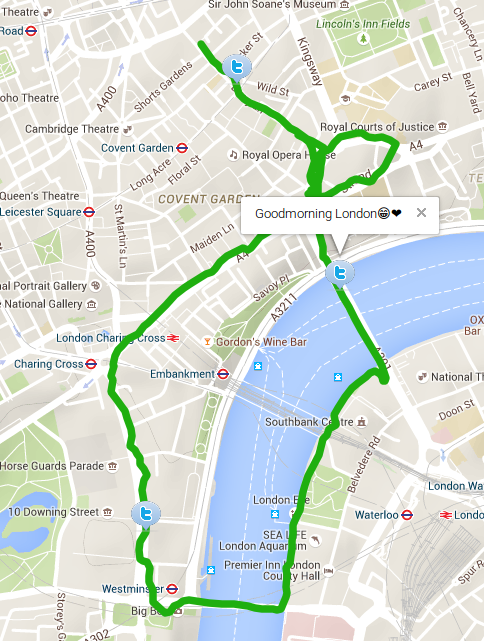
\includegraphics[width=90mm]{tweet.png}
\caption{Some running route in London annotated with location-specific tweets \label{viz:social}}
\end{figure}

\begin{figure}[h]
\centering
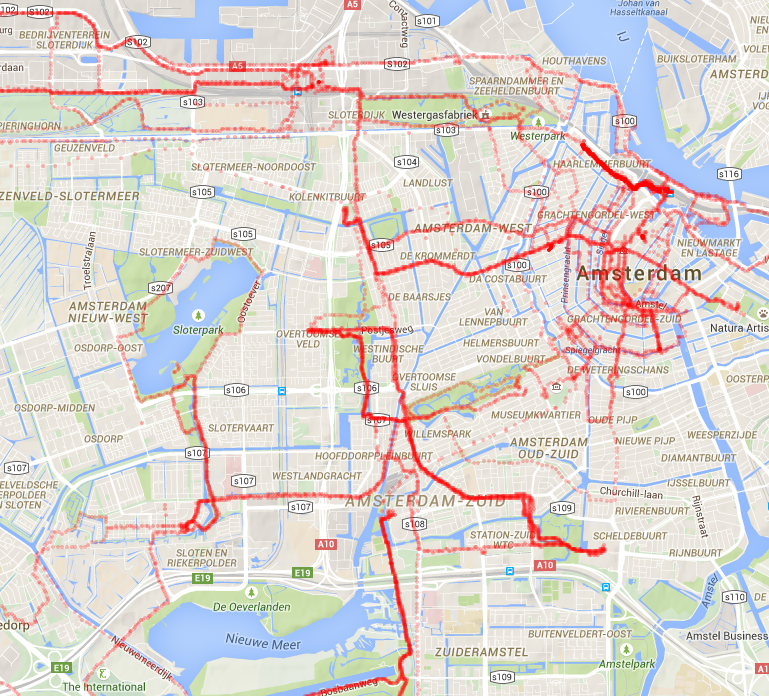
\includegraphics[width=90mm]{popularity.png}
\caption{Popularity of running routes in Amsterdam: paths with bolder color are of higher popularity  \label{viz:popularity}}
\end{figure}

\begin{figure}[h]
\centering
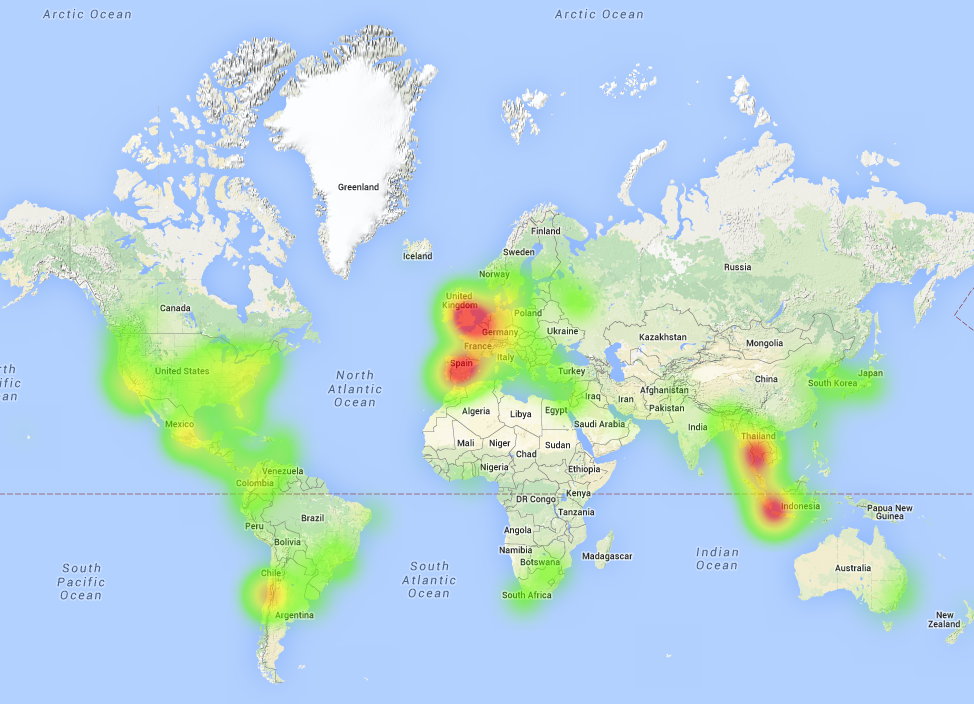
\includegraphics[width=90mm]{global.png}
\caption{Global-wise workout distance heatmap \label{viz:global}}
\end{figure}


\section{Future work}


\section{Conclusion}


%%%%%%%%%%%%%%%%%%%%%%%%%%%%%%%%%%%%%%%%%%%%%%%%%%%%%%%%%%%%%%%%%%%


\end{document}
